%-------------------------------------------------------------------------------
% File: simulation.tex
%       Epidemic Broadcast project documentation.
%
% Author: Marco Pinna, Rambod Rahmani, Yuri Mazzuoli
%         Created on 05/12/2020
%-------------------------------------------------------------------------------
\chapter{Simulation}\label{ch:simulation}
As previously described, two different scenarios were considered, each with a population of $100$ users:
\begin{itemize}
    \item \textbf{Small}: a $10$m x $10$m floorplan, with the transmission
    radius ranging from $1$m to $4.5$m, with a step of $0.5$m, and a Bernoullian
    RV with success probability $p$ ranging from $0.05$ to $0.95$ with steps of
    $0.05$;
    \item \textbf{Big}: a $100$m x $100$m floorplan, with the transmission
    radius ranging from $1$m to $19$m, with a step of $1$m, and a Bernoullian RV
    with success probability $p$ ranging from $0.1$ to $0.9$ with steps of $0.1$;
\end{itemize}
\section*{Methodological Note}\label{Methodological}
In order to analyse all the possible choices for $p$ and $R$, we have to explore the space
formed by the cartesian product of the possible values for each parameter. Every combination 
identifies a scenario, for which we have to approximate performance indexes; in our model
every index is a random variable, and we want to compute its mean value, with a confidence interval
according to a specific confidence level (at least 95\%). 
We do not have enough details to identify the probability distribution of those variables, and 
we are not even sure that they will be symmetric, so we chose to estimate the mean value of every 
distribution by the sample mean and also by the sample median.
We know that sample mean and sample median converge to the same value for a large number
of samples; we simply want to plot the one with the small confidence interval, and we cannot know
\texttt{a priori} which one will be.
For confidence intervals, we chose algorithms that do not require to know the distribution of the
samples; in order to apply those algorithms we only have to verify that our distributions have
limited variance. We can ensure that because:
\begin{itemize}
    \item the \textbf{broadcast time} is bounded from below (because it cannot be less than 1) and from above
        (see \texttt{single queue configuration})
    \item the \textbf{percentage of covered users} is bounded between 0.01 (1\%) to 1 (100\%)
    \item the \textbf{number of collisions} is bounded from below (because it cannot be less than 0) and
        from above by the value 2305 for a floorplan with 100 hosts. The formula for the upper bound can be found in appendix D, toghether with its derivation.
\end{itemize} 

%TODO I think a verb is missing
For each of the scenarios, the floorplan coverage, the
broadcast duration and the number of collisions are mesured and plotted in graphs in order to 
extrapolate insighs about the behaviour of the system.\\
In order to achieve statistically significant results with a minimum accuracy of
$95$\%, each scenario configuration -- with the same parameters -- was run 200 times; then, mean and median values of the performance
indexes were computed, along with their confidence intervals.
\section{Big}\label{sec:big}
\subsection{Coverage}\label{ssec:coverage}
Figure \ref{fig:floorplancoverage1} shows the floorplan coverage achieved as a
function of the success probability $p$, for different values of
the transmission radius $R$. \\
As we can observe, the coverage is maximum
for lower values of $p$; this is due to the fact that a low transmission
probability minimizes the number of collisions, increasing the number of correct
transmissions. For values of $R < 8$ we observe an almost linear behaviour:
collisions are almost absent with such a small transmission radius; therefore,
variations of the value of $p$ do not play a fundamental role as far as total coverage is
concerned. For $R \geq 8$ the achievable coverage
decreases with the increase of $p$, but quite slowly and also it does not
degenerate to $0$; instead it reaches a value between $10$\% and $40$\%.
\begin{figure}[H]
    \begin{center}
        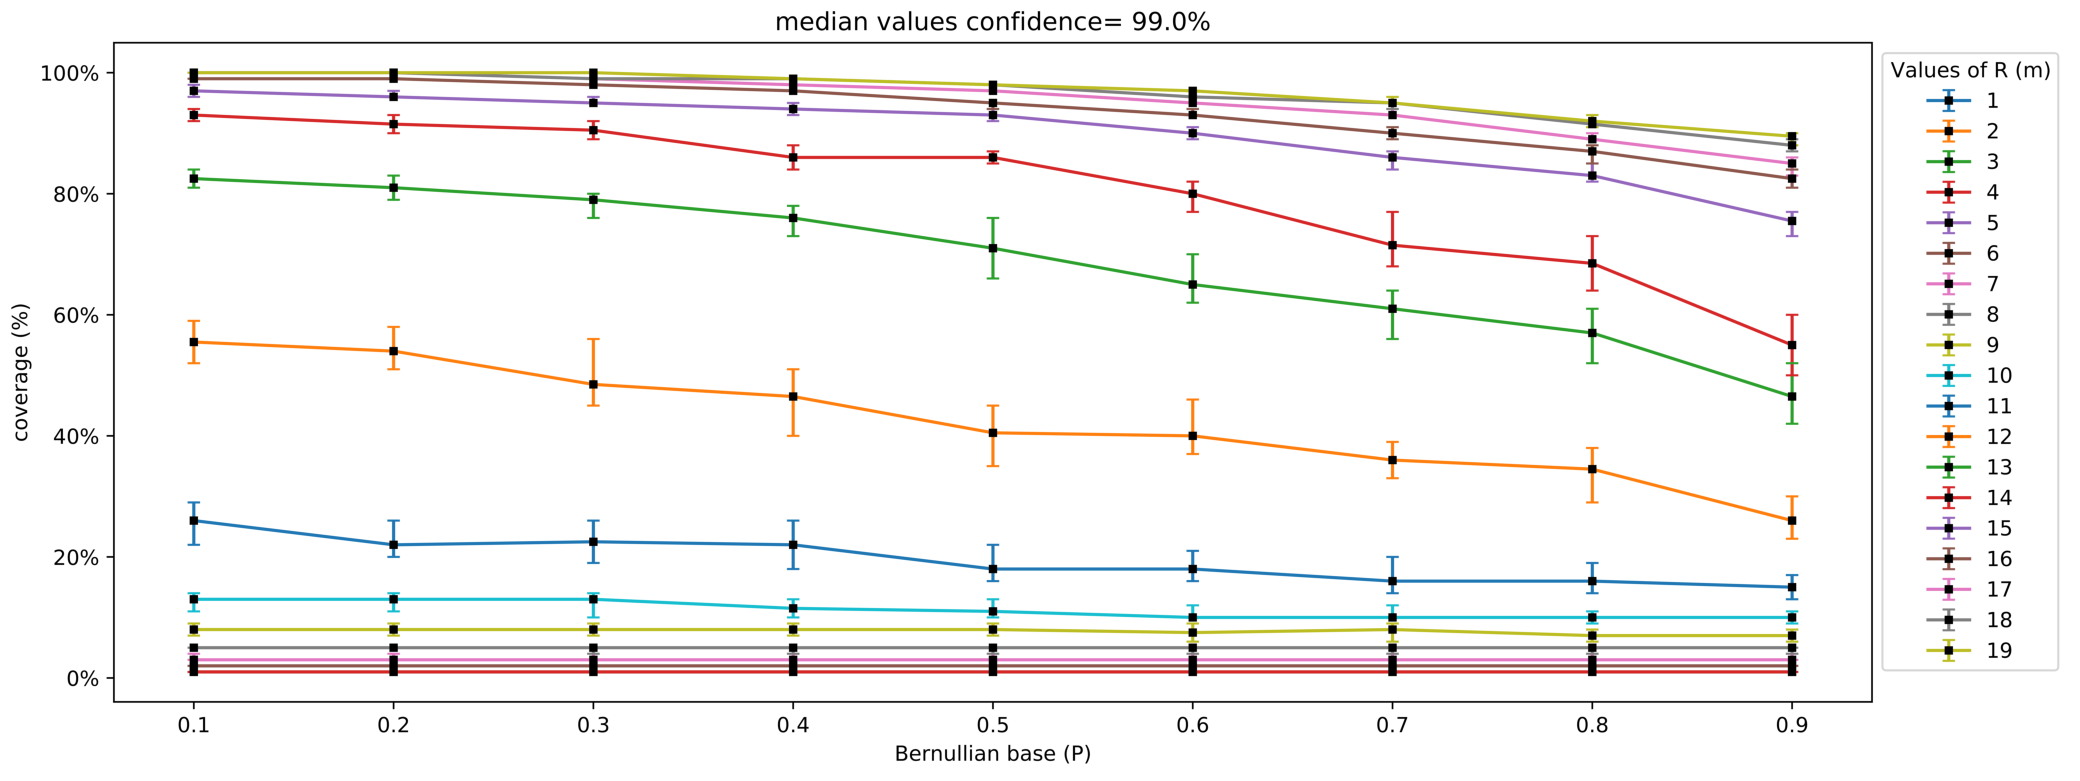
\includegraphics[scale=.42]{img/Big_CovP_median.pdf}
    \end{center}
    \vspace*{-0.5cm}
    \caption{Floorplan coverage as a function of $p$ for different values of $R$}
    \label{fig:floorplancoverage1}
\end{figure}
\noindent
For values of $R$ between $11$ and $15$, the number of collisions has a strong
effect on the coverage percentage; this effect tends to decrease for larger
values of $R$; we know as a matter of fact that for $R \to L\sqrt{2}$ the
coverage tends to $100$\%, independently of any other parameter.\\
\\
Figure \ref{fig:floorplancoverage2} shows the floorplan coverage achieved as a
function of the transmission radius $R$, for different values of the success probability $p$. As expected, accordingly with the previous plot, the
final coverage of the flooplan is deeply influenced by the transmission range $R$.
\begin{figure}[H]
    \begin{center}
        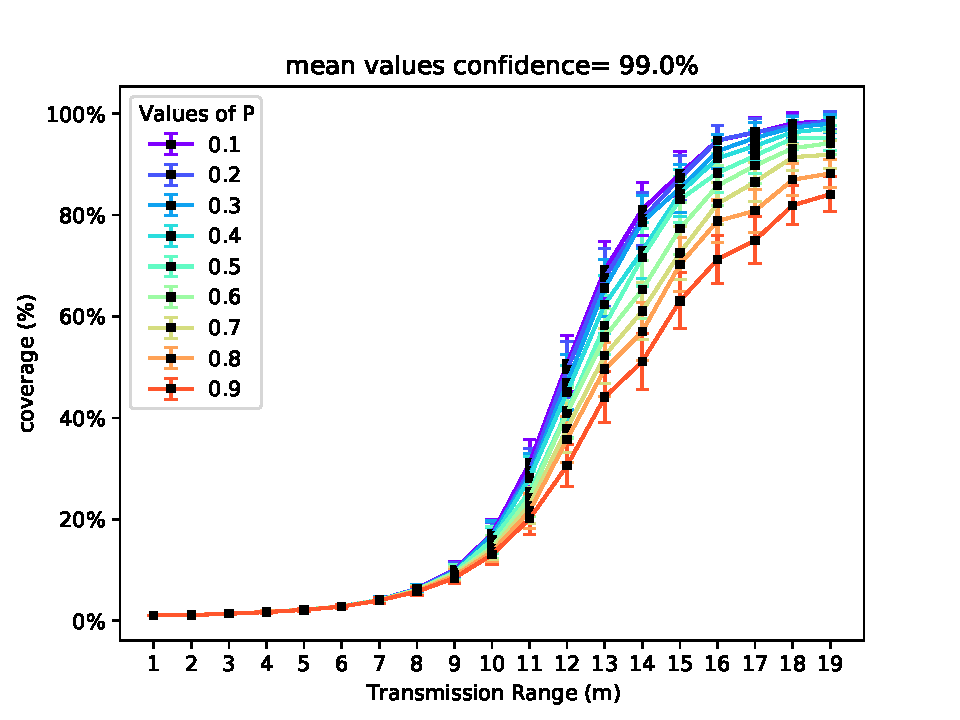
\includegraphics[scale=.75]{img/Big_CovRange_mean.pdf}
    \end{center}
    \vspace*{-0.5cm}
    \caption{Floorplan coverage as a function of $R$ for different values of $p$}
    \label{fig:floorplancoverage2}
\end{figure}
\noindent
%TODO it's better to rephrase and remove 'exponentially' as coverage slows down immediately after r=12 and we ourselves say that it is in fact a sigmoid, not an exponential
In this second plot we can observe that the coverage increases exponentially
with the transmission range. When the transmission range becomes large
($> 16$m), the coverage tends to $100$\%. We recognized the shape of the
sigmoid\footnote{https://mathworld.wolfram.com/SigmoidFunction.html} function,
which can be express as an hyperbolic tangent ($\tanh$); this function is always
increasing and can be manipulated to remain between $0$ and $1$ (like the
parameter we want to fit). A good fit for this curve is given by:
\begin{equation*}
    C = \frac{1+\tanh(aR+b)}{2}
\end{equation*}
where $C$ is the floorplan coverage, $R$ the transmission radius, and $a$ and
$b$ depend on $p$ as shown in the following table:
\begin{center}
\begin{tabular}{ | m{1cm} | m{4cm}| m{4cm} | }
\hline
$p$&$a$&$b$\\
\hline
$0.1$&$0.3628314535334378$&$4.356732935967713$\\
\hline
$0.2$&$0.3572920723369711$&$4.3206795324164835$\\
\hline
$0.3$&$0.34371134773480694$&$4.193385575628803$\\
\hline
$0.4$&$0.3217942874156316$&$3.9814759531755515$\\
\hline
$0.5$&$0.3091448275788839$&$3.88645016495332$\\
\hline
$0.6$&$0.2809863550485405$&$3.6000814495973996$\\
\hline
$0.7$&$0.25932462296148107$&$3.3996924196436975$\\
\hline
$0.8$&$0.23603288616377227$&$3.1648817545125527$\\
\hline
$0.9$&$0.20917405109220505$&$2.929033169711656$\\
\hline
\end{tabular}
\end{center}
\subsection{Duration}
This following figure shows the plot of the duration of the simulation (in
seconds) as a function of $p$, for different values of $R$.
\begin{figure}[H]
    \begin{center}
        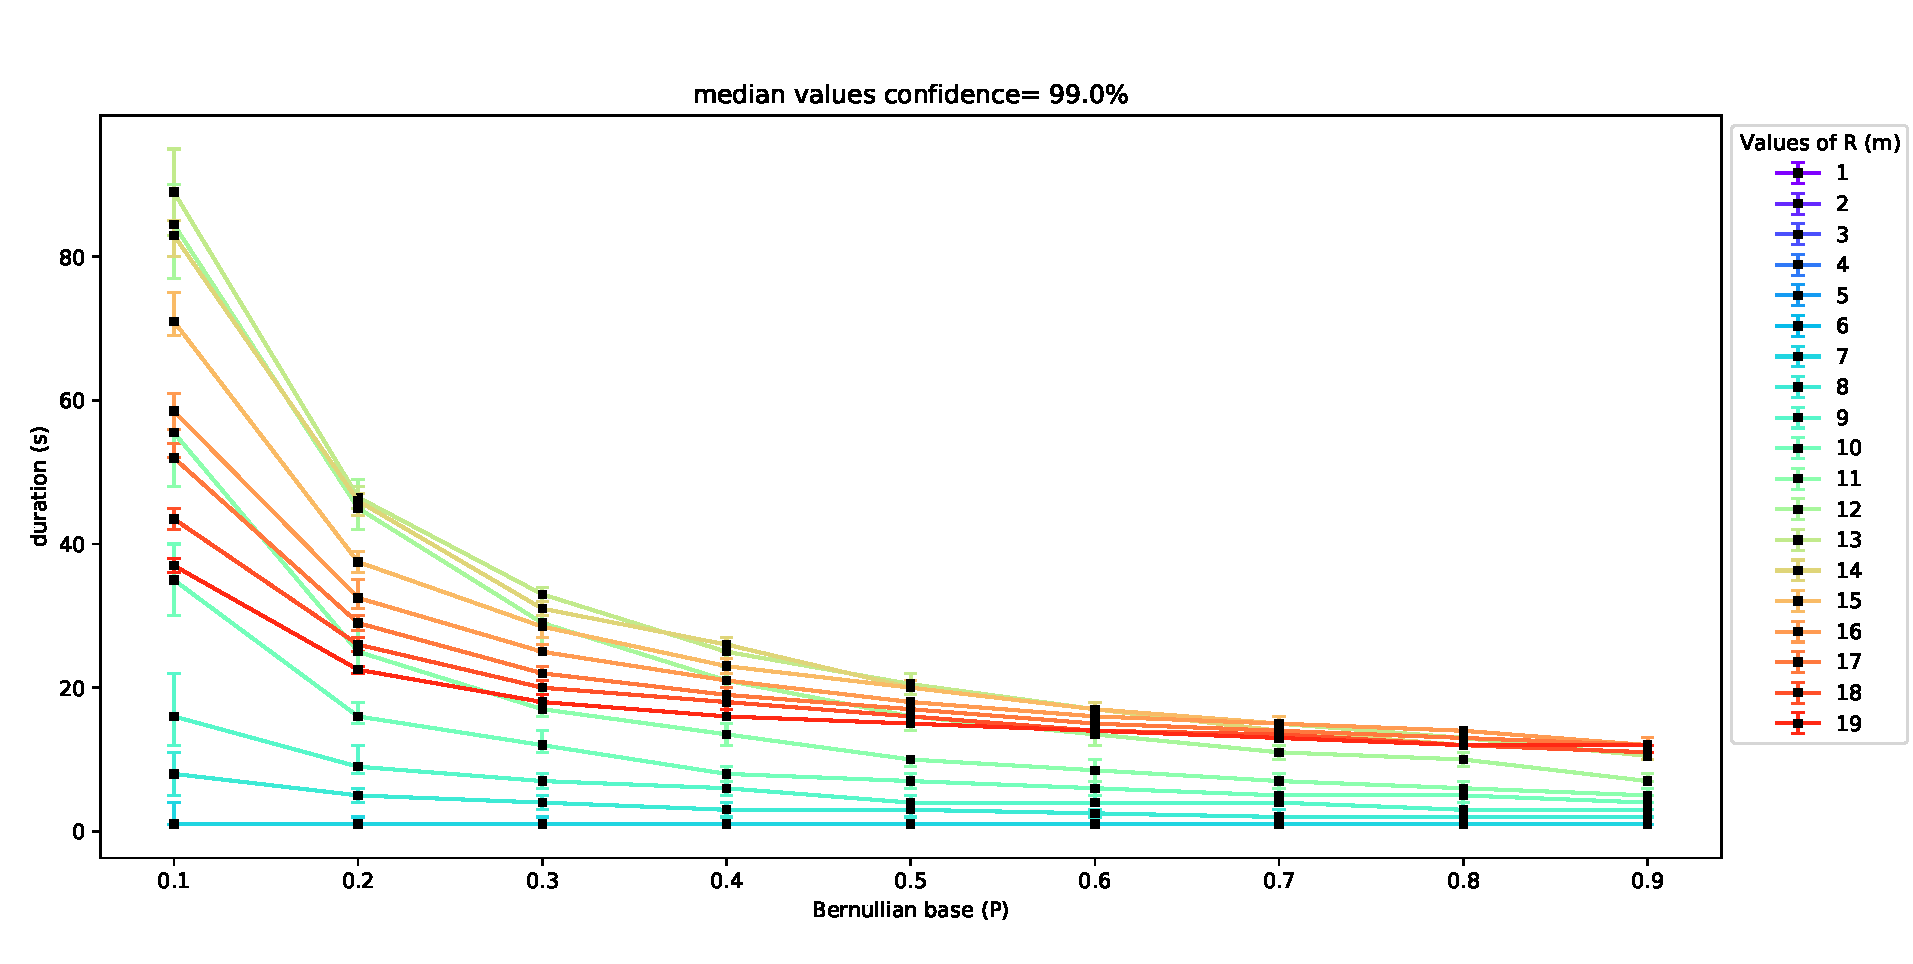
\includegraphics[scale=.51]{img/Big_DurP_median.pdf}
    \end{center}
    \vspace*{-0.5cm}
    \caption{Simulation duration as a function of $p$ for different values of $R$}
    \label{fig:floorplancoverage3}
\end{figure}
\noindent
The simulation duration increases for lower values of $p$; this behaviour can be
explained as a consequence of two main factors:
\begin{itemize}
    \item the probability of retransmission is low, so nodes will spend most
    time slots waiting, without actually transmitting;
    \item with a smaller number of collisions, a higher number of nodes is
    reached; reaching a higher number of nodes requires a higher number of
    retransmissions.
\end{itemize}
We tried to interpolate the curves shown in Figure \ref{fig:floorplancoverage3}
with an hyperbolic function, because it fits well the parameters we want to
model; first of all, the hyperbole tends to infinity as $p$ tends to $0$, and
this is coherent with the reality, because if the probability of retransmission
becomes low, then the duration keeps increasing. If instead $p$ gets close to
$1$, the duration time tends to its minimum. We fit those shapes using:
\begin{equation*}  
    D = \frac{a}{P}+b 
\end{equation*}
where $D$ is the duration of the simulation, $p$ the probability of
retransmission, and $a$ and $b$ depend on $R$ as specified in the following
table:
%TODO too many digits. Better to reformat as the wall of text is not exactly pretty
\begin{center}
\begin{tabular}{ | m{1cm} | m{5cm}| m{5cm} | }
\hline
$R$&$a$&$b$\\
\hline
$1$&$2.4046845625846913$ e-09&$0.999999999244136$\\
\hline
$2$&$2.4046845625846913$ e-09&$0.999999999244136$\\
\hline
$3$&$0.7313966348173997$&$0.9495446821974095$\\
\hline
$4$&$1.3471717522270503$&$0.9454326532617134$\\
\hline
$5$&$1.7744177255115228$&$1.08724762049118$\\
\hline
$6$&$4.652279267805434$&$1.0487610714204172$\\
\hline
$7$&$9.586489452244717$&$1.088347295851843$\\
\hline
$8$&$15.841670397411658$&$1.0643797063994824$\\
\hline
$9$&$28.264640360031194$&$0.49558107430696624$\\
\hline
$10$&$43.141734847778814$&$0.22815570364285975$\\
\hline
$11$&$64.55944043148898$&$-0.07517936077209139$\\
\hline
$12$&$86.56257725232254$&$-0.09919809415424388$\\
\hline
$13$&$89.72686483087844$&$1.2578386401845827$\\
\hline
$14$&$82.15919574473708$&$3.0965825999956778$\\
\hline
$15$&$67.95268283187643$&$5.415446394742158$\\
\hline
$16$&$56.442159145137495$&$6.991880399220213$\\
\hline
$17$&$45.71412729773696$&$7.548465010848107$\\
\hline
$18$&$39.164500694866284$&$7.991652317096266$\\
\hline
$19$&$29.71836400235831$&$9.075854630828385$\\
\hline
\end{tabular}
\end{center}
To be able to compute the correct values the first two entries for $a$ and $b$,
a larger dataset is needed; as a matter of fact, if the transmission range is
too short nodes can not communicate: they are not in reach by each others.\\
\\
The following plot shows the duration of the simulation (in seconds) as a
function of $R$, for different values of $p$.
\begin{figure}[H]
    \begin{center}
        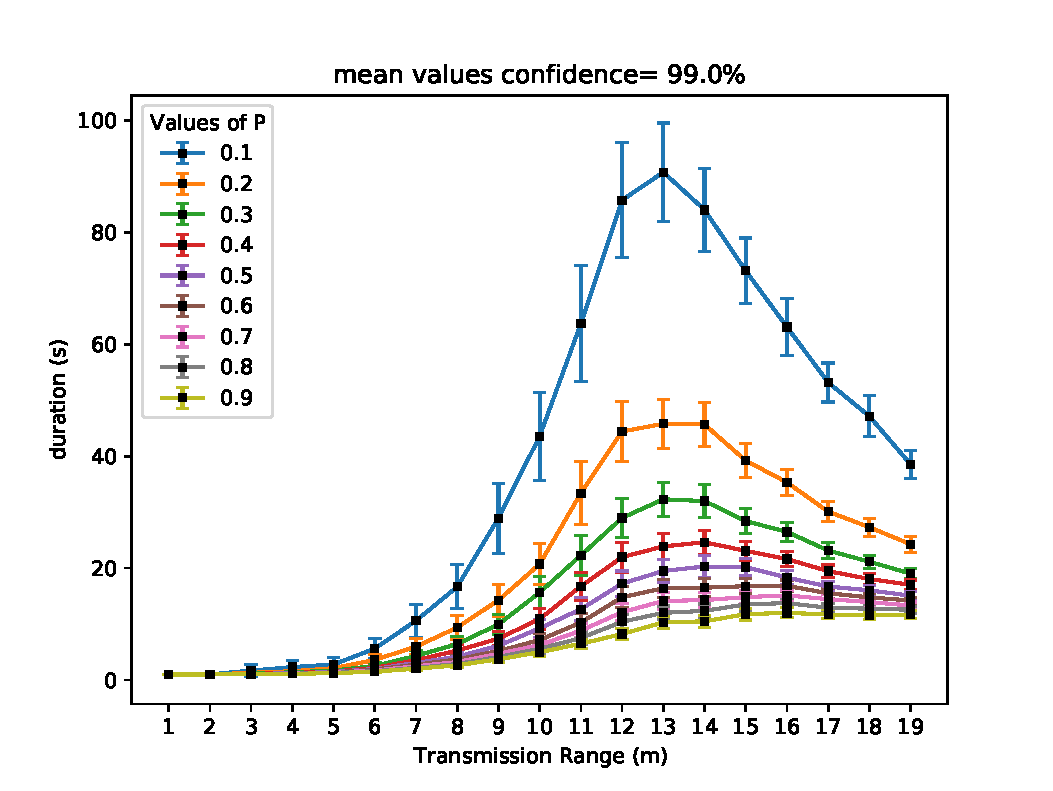
\includegraphics[scale=.7]{img/Big_DurRange_mean.pdf}
    \end{center}
    \vspace*{-0.5cm}
    \caption{Simulation duration as a function of $R$ for different values of $p$}
    \label{fig:floorplancoverage4}
\end{figure}
\noindent
The duration of the simulation tends to increase with the transmission range
reaching a peak around $13$m; the maximum value depends on the probability of
retransmission ($p$);
This is an interesting result, and can be explained by:?%todo
\subsection{Collisions}
This plot show the Number of collisions in function of P, for different values of R.
\begin{figure}[H]
    \begin{center}
        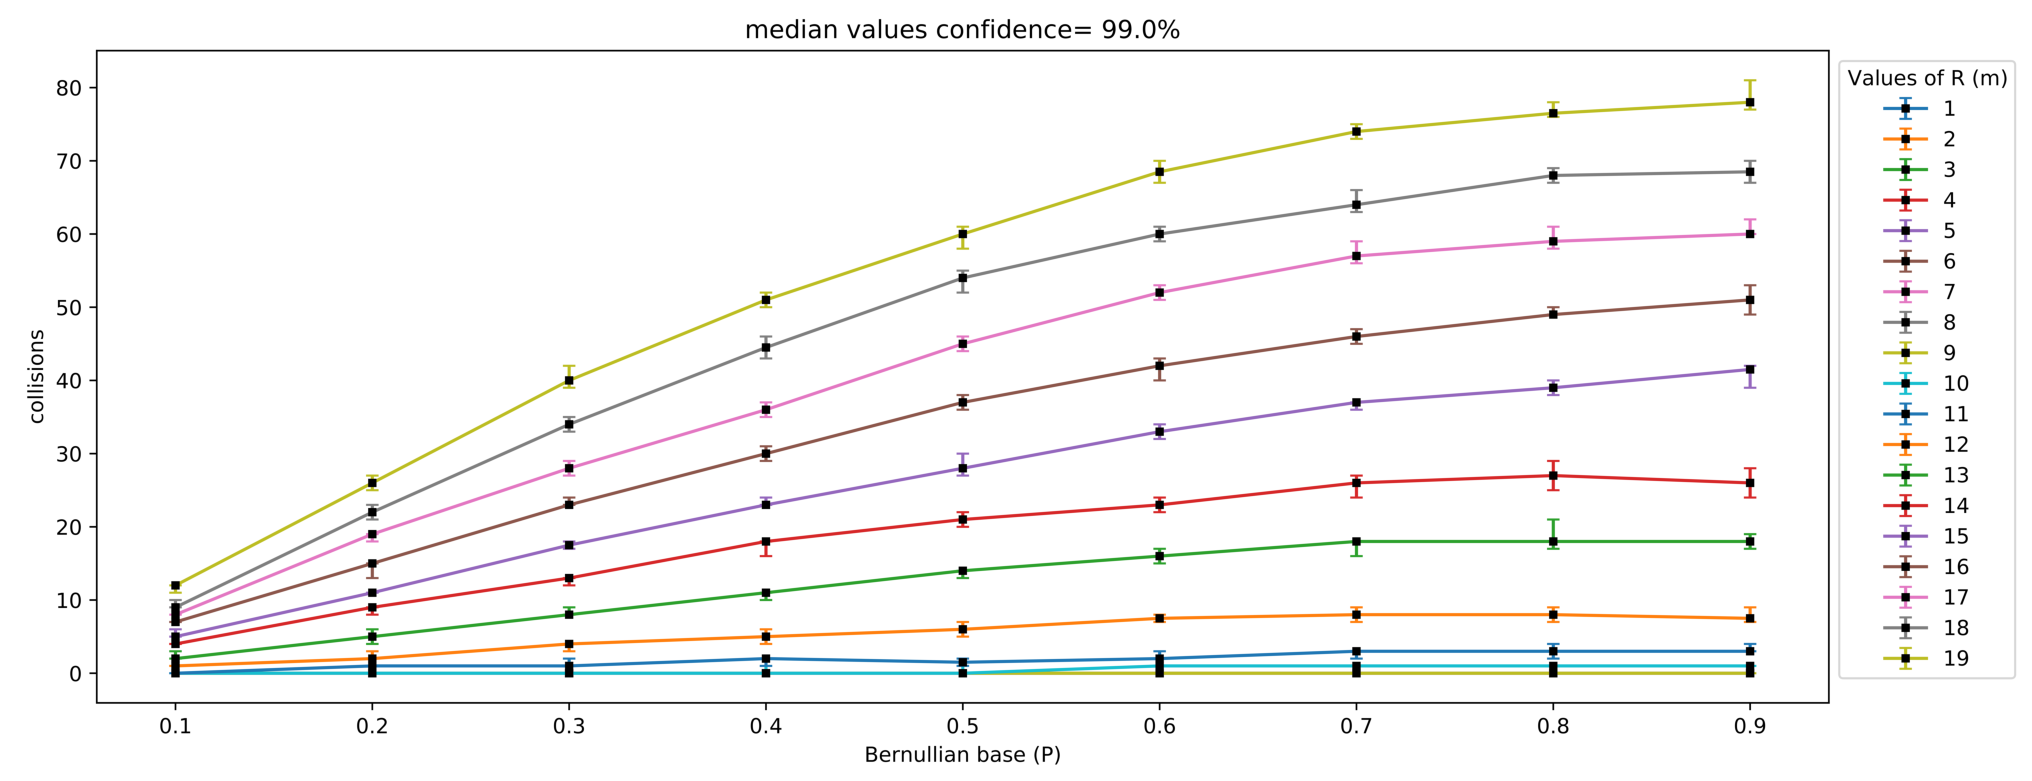
\includegraphics[scale=.4]{img/Big_CollP_median.pdf}
    \end{center}
    \vspace*{-0.5cm}
    \caption{Caption this}
    \label{fig:floorplancoverage5}
\end{figure}
\begin{figure}[H]
    \begin{center}
        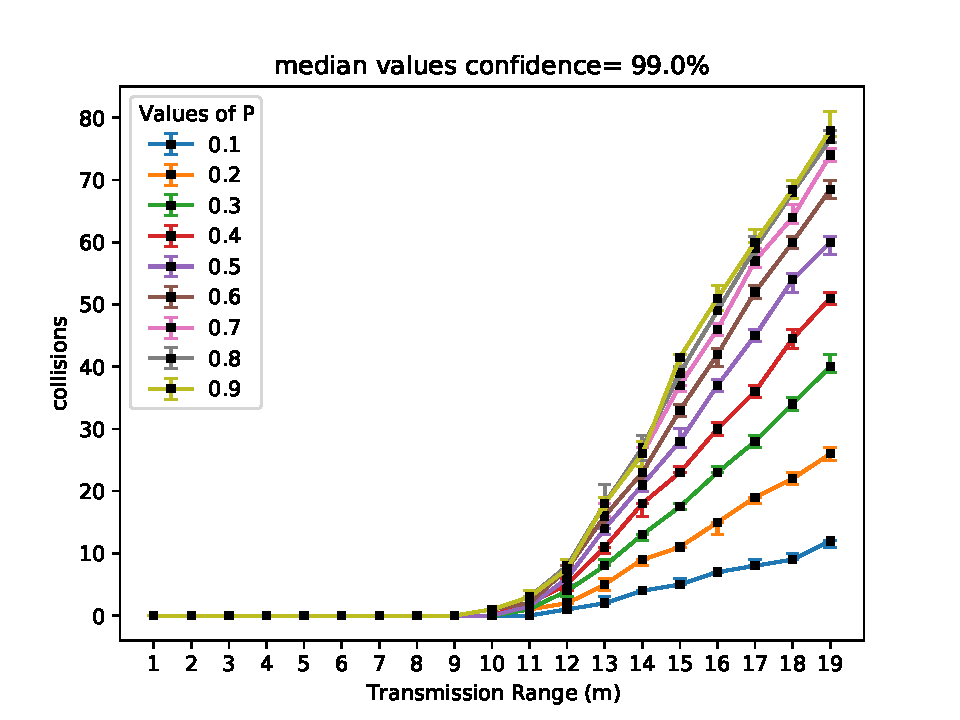
\includegraphics[scale=.7]{img/Big_CollRange_median.pdf}
    \end{center}
    \vspace*{-0.5cm}
    \caption{Caption this}
    \label{fig:floorplancoverage6}
\end{figure}

\section{Comparison between KPIs and graph properties}

Some of the results shown in the previous section can be better understood when compared with some properties of the graphs associated with the configurations of the hosts.\\
In particular, three properties of the graphs have been studied:

\begin{itemize}
	\item the \texttt{reach}, defined as the number of nodes that can be reached from host (vertex) 0. More formally, let $H$ be the connected component containing host 0 of the initial graph $G$, i.e. the induced subgraph in which any vertex is connected to vertex 0. The \texttt{reach} is the \textit{order} of $H$.
	\item the \texttt{eccentricity}, already defined in \ref{sec:graphModelForWirelessSystems}
	\item the number of \texttt{safe nodes}, which has been defined for simulations with $p=1$ as the number of nodes that correctly receive the message. Systems with $p=1$ are completely deterministic and therefore the number of \textit{safe nodes} only depends on the topology of the network.
\end{itemize}

\subsection{Coverage, reach and safe nodes}

In \ref{ssec:coverage} results about the coverage were shown and it was hypothesized that this index, as function of $R$, might have a sigmoidal trend.\\
Let us consider the limit case where $p \to 0$.\\
As $p$ approaches 0, during each slot it becomes less and less likely for an active node to transmit the message. On the other hand, smaller values of $p$ lower the probability of collisions even more.\\
For values of $p$ really close to 0, it is easy to imagine that there will be basically no collisions; at the same time, every node belonging to the connected component of node 0 will sooner or later receive the message with a probability of 1.\\
\begin{figure}[H]
    \begin{center}
        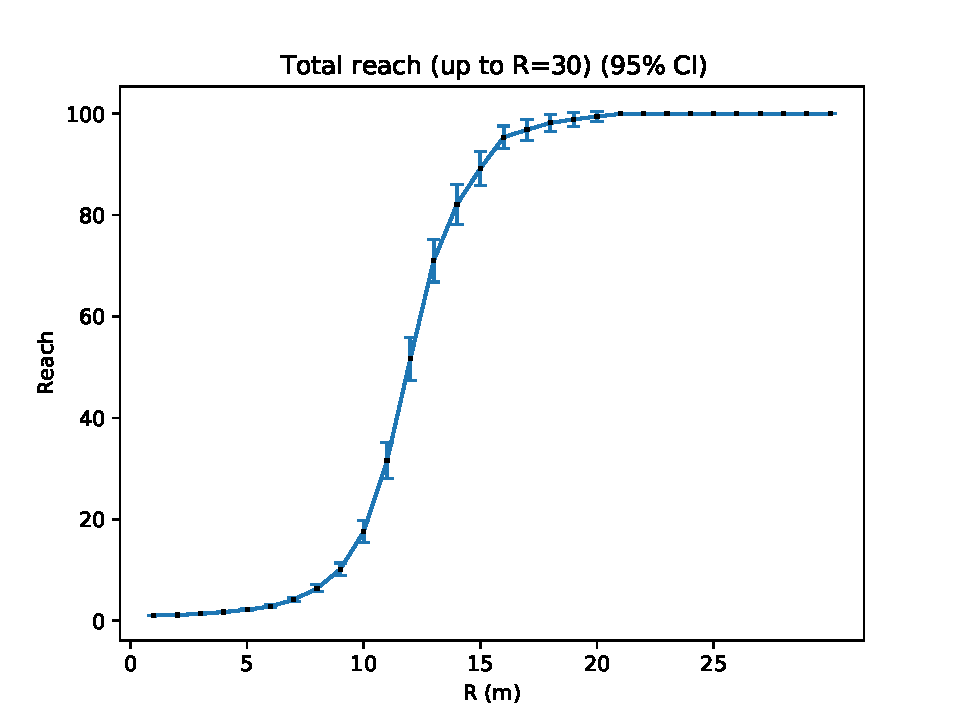
\includegraphics[scale=.6]{img/graphAnalysisTotal_reachR30.pdf}
    \end{center}
    \vspace*{-0.5cm}
    \caption{Average reach of a graph as function of R}
    \label{fig:reachR30}
\end{figure}
\hfill \break
Figure \ref{fig:reachR30} shows the average reach from node 0, as function of $R$, in a graph with 100 nodes. Values for $R>30$ are not shown as the function plateaus at a value of 100. \\
Various sigmoid functions have been tested to fit the experimental values for the \textit{reach}, and the most appropriate one was found to be
\hfill \break
\begin{equation}\label{eq:reachSigmoidParametric}
	S(R) = \frac{1}{N} + \frac{N-1}{N}\cdot\frac{1+tanh(b(R-a))}{2}
\end{equation}
\hfill \break
where $N$ is the number of nodes in the graph, $a$ controls to the abscissa of the inflection point and $b$ controls how steep the increase is.\\
The correct value for $a$ can be found examining the data in fig. \ref{fig:reachR30} and observing that they show an inflection point for $R=12m$. With regard to parameter $b$, trial and error showed that its value lies between $0.36$ and $0.37$. In fact, a value equal to $e^{-1} \approx 0.36788$ fits the data very well.\\
% and it makes sense in the presence of a hyperbolic tangent function
A closed form for the \textit{reach}, and therefore for total coverage when $p \to 0$, would then be
\hfill \break
\begin{equation}\label{eq:reachSigmoid}
	C_{0}(R) = \frac{1}{100} + \frac{99}{100}\cdot\frac{1+tanh(e^{-1}(R - 12))}{2}
\end{equation}
\hfill \break
It is reasonable to think that $a$ depends both on the number of nodes and on the total area of the floorplan, while $b$ might be a constant that does not depend on any quantity of the system.\\
\hfill \break
Let us now consider the limit case where $p \to 1$.\\
The closer $p$ gets to $1$, the more the system approaches a deterministic behaviour where each active host broadcasts the message as soon as it receives it.\\
When $p=1$ the number of node that correctly receive the message during the broadcast can be computed by knowing only the topology of the network.\\
\begin{figure}[H]
    \begin{center}
        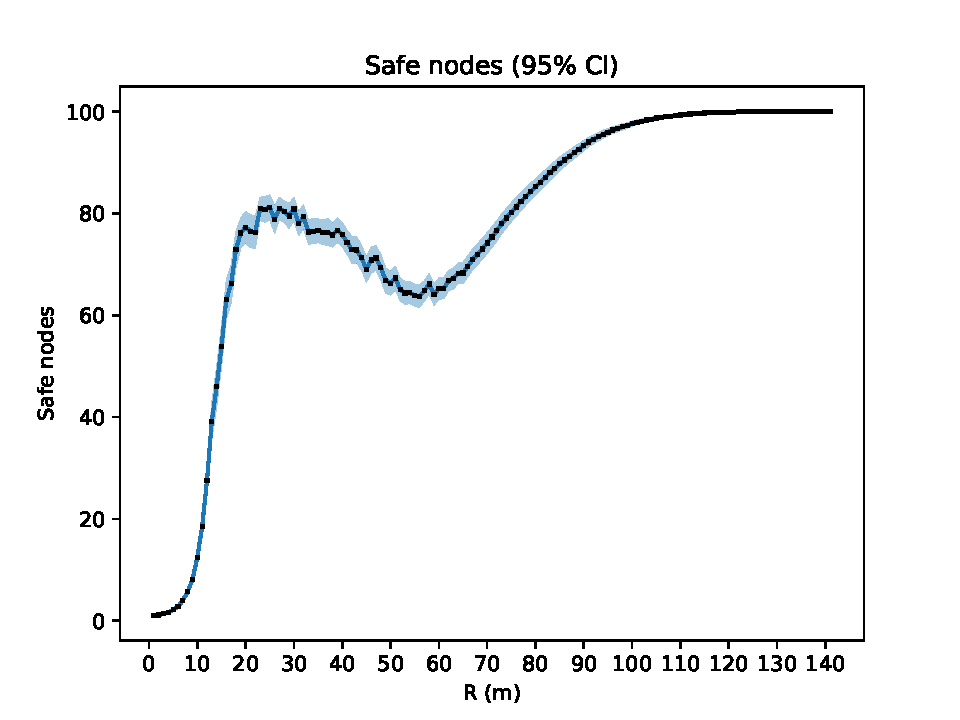
\includegraphics[scale=.6]{img/graphAnalysisSafe_nodes.pdf}
    \end{center}
    \vspace*{-0.5cm}
    \caption{Average number of safe nodes of a graph as function of R}
    \label{fig:safeNodes}
\end{figure}
\hfill \break
Figure \ref{fig:safeNodes} shows the average number of safe nodes during a broadcast starting from node 0, as function of $R$, in a graph with 100 nodes.\\
It is clear that this function does not have a sigmoidal trend, except for low values of $R$, up to about 25 metres, where the number of safe nodes reaches about 80. This is consistent with the trend of the curve for $p=0.9$ in Figure \ref{fig:floorplancoverage2} shown in the previous section.\\
For $R > 25$ increasing the radius yields negative returns: the average number of safe nodes decreases until $R$ reaches about 55 metres. This is likely to be due to the fact that the increase in the number of collision takes over on the increase of reachable nodes. This is consistent with the hypothesis made in Chapter \ref{ch:overview} when analysing the impact of $R$ on the KPIs.\\
For $R > 55$ the number of safe nodes starts increasing again, probably because host 0 starts having more and more neighbours when the broadcast begins (and none of them detects a collision as host 0 is the only one transmitting during the first slot).\\ The quantity asymptotes to the total number of nodes and for $R > \sqrt{2}{\cdot}L$ it is identically equal to it since, wherever the starting node would happen to be placed, it would cover the whole area during its first transmission slot.\\
\hfill \break
These considerations show that the coverage as function of $R$, although it might resemble a sigmoid for different values of $p$ (and could probably be approximated well enough by it for realistic value of the transmission range), is probably more complex than that; for a certain range of values for R, the increase in the number of collision starts having a heavier role in the number of reached hosts.\\
A closed formula for the number of safe nodes when $p=1$ has not been found yet but, assuming it is $C_{1}(R)$, then a reasonable form for the coverage function could be the following:
\begin{equation}\label{eq:coverageClosedForm}
C(R, p) = (1-p)\cdot C_{0}(R) + p\cdot C_{1}(R)
\end{equation}

\subsection{Broadcast time and eccentricity}
In \ref{sec:graphModelForWirelessSystems} the eccentricity $\epsilon$ of a graph was introduced, defined as the distance from node 0 to the furthest connected node, let it be $u$.\\
If we imagine the message spreading from host 0 outwards along the various paths of the graph, it is easy to guess that, on average, the path that will take the longest to be covered will be the one that leads to node $u$ and this path will have, by definition, a number of edges equal to the eccentricity.\\
\begin{figure}[H]
	\begin{minipage}{.5\textwidth}
        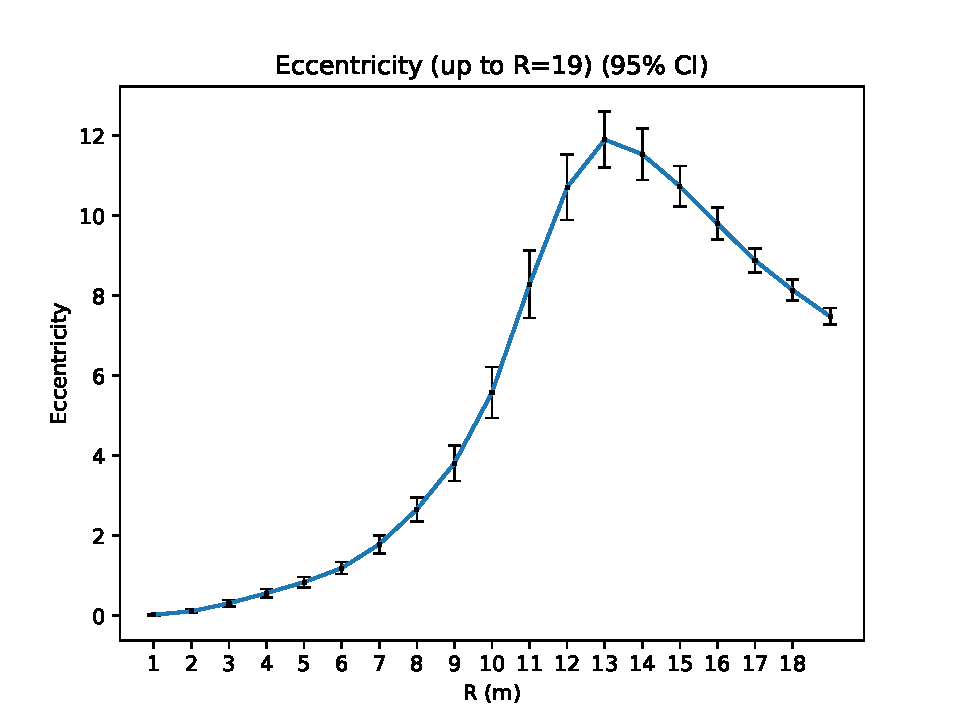
\includegraphics[scale=.5]{img/graphAnalysisEccentricityR19.pdf}
        \begin{center}
            a) Eccentricity as function of R
        \end{center}
	\end{minipage}
	\begin{minipage}{.5\textwidth} 
		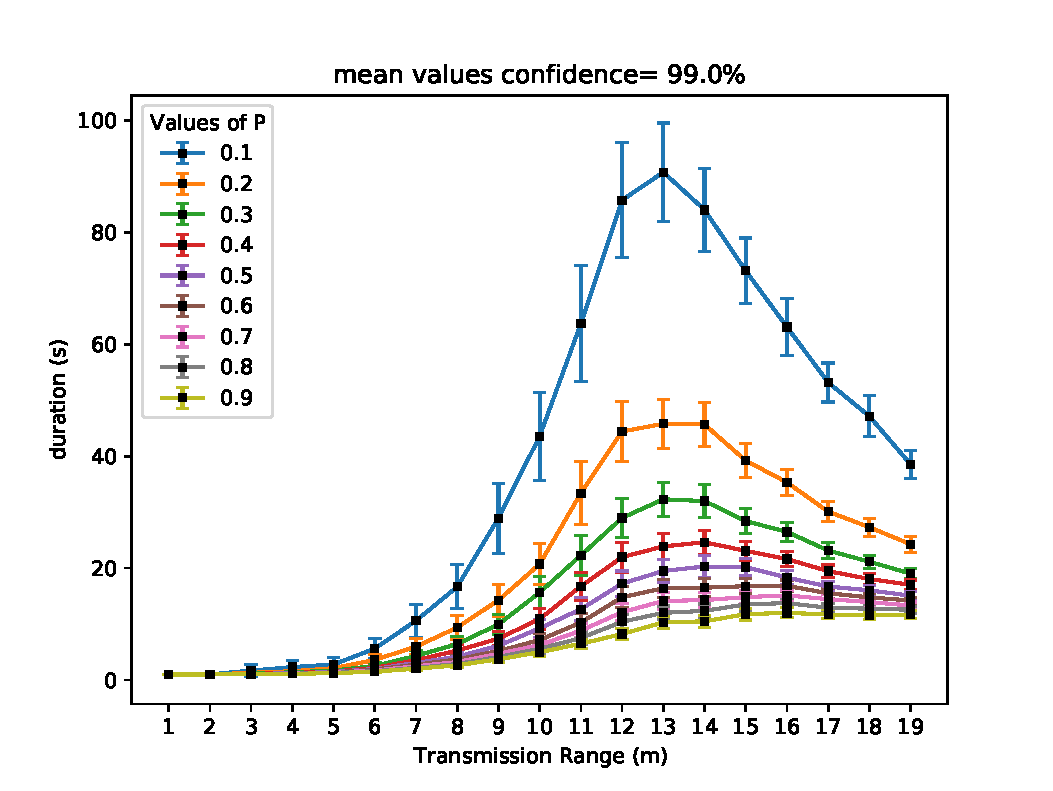
\includegraphics[scale=.5]{img/Big_DurRange_mean.pdf}
		\begin{center}
            b) Broadcast time as function R
        \end{center}
	\end{minipage}
	\caption{}
    \label{fig:eccentricityDuration}
\end{figure}
\hfill \break
Fig. \ref{fig:eccentricityDuration} shows the average eccentricity of a graph with 100 nodes, with respect to node 0, as function of $R$ and once again the experimental data for the duration, for convenience of comparison.\\
The curves on the right clearly resemble the one on the left, minus a scaling factor.\\
The spacing between the duration curves might suggest that this scaling factor is the inverse of the corresponding $p$. This would make complete sense because the average time a message takes to travel along a path of $n$ hops is $n \cdot \frac{1}{p}$ (see \ref{ssec:singlequeue}).\\
In fact, while the spacing does indeed suggest an inverse dependency on $p$, the actual values turn out to be about 20\% smaller. The existence of this additional $\sim 0.8$ scaling factor could be motivated as follows:\\
the eccentricity of a graph gives information about the longest path from a node to the furthest node $u$, but does not say anything about the number of paths of that length. In the graph there might very well be different paths of length $\epsilon$ that connect node 0 to $u$, either completely disjunct or with some nodes in common and ``forks", ``branch-ins" and ``branch-outs". If these paths happens to be disjunct, node $u$ will receive the message as soon as it arrives from the ``fastest" one. 

\begin{wrapfigure}{r}{0.45\textwidth}
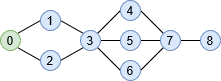
\includegraphics[width=1\linewidth]{img/branchIn.png} 
\caption{Example of graph with multiple shortest path of lenght $\epsilon$}
\label{fig:branchIn}
\end{wrapfigure}

If the paths happen to have nodes in common, as it is the case in fig. \ref{fig:branchIn}, every time there is a ``branch-in" ($[1,2]{\to}3$ or $[4,5,6]{\to}7$ in the figure) there is a possibility that the message will have a speed ``boost" with respect to its average speed along a single queue and also a possibility that its progress will be interrupted by a collision.



